\chapter{Evolutionary algorithms}


%====================================================================================================
\section{Biological evolution}

%--------------------------------------------------------------------------------------------------
\subsection{Dawrwin theory and its modern form}
The scientific theory of evolution by natural selection was conceived independently by
Charles Darwin and Alfred Russel Wallace in the mid-19th century and was set out in detail in
Darwin's book On the Origin of Species.
Evolution by natural selection was first demonstrated by the observation that more offspring are
often produced than can possibly survive. 
This is followed by three observable facts about living organisms:
\begin{enumerate}
	\item  tphenotypic variatio - nraits vary among individuals with respect to their morphology,
		physiology and behaviour, 
	\item ddifferential fitnes - sifferent traits confer different rates of survival 
		and reproduction, 
	\item heritability of fitness - traits can be passed from generation to generation.
\end{enumerate}
Thus, in successive generations members of a population are more likely to be replaced by
the progenies of parents with favourable characteristics that have enabled them to survive and 
reproduce in their respective environments. 
In the early 20th century, other competing ideas of evolution such as mutationism and orthogenesis
were refuted as the modern synthesis reconciled Darwinian evolution with classical genetics,
which established adaptive evolution as being caused by natural selection acting on
Mendelian genetic variation.

All life on Earth shares a last universal common ancestor (LUCA) that lived approximately
3.5–3.8 billion years ago.
The fossil record includes a progression from early biogenic graphite, to microbial mat fossils,
to fossilised multicellular organisms.
Existing patterns of biodiversity have been shaped by repeated formations of new species 
(speciation), changes within species (anagenesis) and loss of species (extinction) throughout the 
evolutionary history of life on Earth.
Morphological and biochemical traits are more similar among species that share a more recent 
common ancestor, and can be used to reconstruct phylogenetic trees.

Evolution in organisms occurs through changes in heritable traits—the inherited characteristics of
an organism. 
In humans, for example, eye colour is an inherited characteristic and an individual might inherit 
the "brown-eye trait" from one of their parents.
Inherited traits are controlled by genes and the complete set of genes within an organism's genome
(genetic material) is called its genotype.

The complete set of observable traits that make up the structure and behaviour of an organism is
called its phenotype. 
These traits come from the interaction of its genotype with the environment. 
As a result, many aspects of an organism's phenotype are not inherited. For example, suntanned skin
comes from the interaction between a person's genotype and sunlight; thus, suntans are not passed
on to people's children.
However, some people tan more easily than others, due to differences in genotypic variation;
a striking example are people with the inherited trait of albinism,
who do not tan at all and are very sensitive to sunburn.

Heritable traits are passed from one generation to the next via DNA, a molecule that encodes 
genetic information. DNA is a long biopolymer composed of four types of bases.
The sequence of bases along a particular DNA molecule specify the genetic information,
in a manner similar to a sequence of letters spelling out a sentence.
Before a cell divides, the DNA is copied, so that each of the resulting two cells will inherit the
DNA sequence. Portions of a DNA molecule that specify a single functional unit are called genes;
different genes have different sequences of bases.
Within cells, the long strands of DNA form condensed structures called chromosomes.
The specific location of a DNA sequence within a chromosome is known as a locus.
If the DNA sequence at a locus varies between individuals, the different forms of this sequence
are called alleles. DNA sequences can change through mutations, producing new alleles.
If a mutation occurs within a gene, the new allele may affect the trait that the gene controls,
altering the phenotype of the organism.
However, while this simple correspondence between an allele and a trait works in some cases, 
most traits are more complex and are controlled by quantitative trait loci
(multiple interacting genes).

Recent findings have confirmed important examples of heritable changes that cannot be explained by
changes to the sequence of nucleotides in the DNA.
These phenomena are classed as epigenetic inheritance systems.
DNA methylation marking chromatin, self-sustaining metabolic loops, gene silencing by RNA 
interference and the three-dimensional conformation of proteins (such as prions) are areas where
epigenetic inheritance systems have been discovered at the organismic level. 
Developmental biologists suggest that complex interactions in genetic networks and communication 
among cells can lead to heritable variations that may underlay some of the mechanics in
developmental plasticity and canalisation.
Heritability may also occur at even larger scales. For example, ecological inheritance through
the process of niche construction is defined by the regular and repeated activities
of organisms in their environment. 
This generates a legacy of effects that modify and feed back into the selection regime of 
subsequent generations.
Descendants inherit genes plus environmental characteristics generated by the ecological
actions of ancestors.
Other examples of heritability in evolution that are not under the direct control of genes 
include the inheritance of cultural traits and symbiogenesis. 
%--------------------------------------------------------------------------------------------------
\subsection{Genetics}
Genetics is a branch of biology concerned with the study of genes, genetic variation, and heredity 
in organisms.

Though heredity had been observed for millennia, Gregor Mendel, Moravian scientist and
Augustinian friar working in the 19th century in Brno, was the first to study genetics 
scientifically.
Mendel studied "trait inheritance", patterns in the way traits are handed down from parents to
offspring.
He observed that organisms (pea plants) inherit traits by way of discrete ``units of inheritance''.
This term, still used today, is a somewhat ambiguous definition of what is referred to as a gene.

Trait inheritance and molecular inheritance mechanisms of genes are still primary principles of
genetics in the 21st century, but modern genetics has expanded beyond inheritance to studying the 
function and behavior of genes.
Gene structure and function, variation, and distribution are studied within the context of the
cell, the organism (e.g. dominance), and within the context of a population.
Genetics has given rise to a number of subfields, including molecular genetics,
epigenetics and population genetics. Organisms studied within the broad field span the domains of
life (archaea, bacteria, and eukarya).

Genetic processes work in combination with an organism's environment and experiences to influence
development and behavior, often referred to as nature versus nurture.
The intracellular or extracellular environment of a living cell or organism may switch gene 
transcription on or off. 
A classic example is two seeds of genetically identical corn, one placed in a temperate
climate and one in an arid climate (lacking sufficient waterfall or rain).
While the average height of the two corn stalks may be genetically determined to be equal, 
the one in the arid climate only grows to half the height of the one in the temperate climate
due to lack of water and nutrients in its environment. 

Modern genetics started with Mendel's studies of the nature of inheritance in plants.
In his paper "Versuche über Pflanzenhybriden" ("Experiments on Plant Hybridization"), 
presented in 1865 to the Naturforschender Verein (Society for Research in Nature) in Brünn,
Mendel traced the inheritance patterns of certain traits in pea plants and described them
mathematically.
Although this pattern of inheritance could only be observed for a few traits, Mendel's work 
suggested that heredity was particulate, not acquired, and that the inheritance patterns of
many traits could be explained through simple rules and ratios.

The importance of Mendel's work did not gain wide understanding until 1900, after his death,
when Hugo de Vries and other scientists rediscovered his research.
William Bateson, a proponent of Mendel's work, coined the word genetics in 1905
(the adjective genetic, derived from the Greek word genesis, "origin", predates the noun and was
first used in a biological sense in 1860).
Bateson both acted as a mentor and was aided significantly by the work of other scientists from
Newnham College at Cambridge, specifically the work of Becky Saunders, Nora Darwin Barlow, and 
Muriel Wheldale Onslow.
Bateson popularized the usage of the word genetics to describe the study of inheritance in his
inaugural address to the Third International Conference on Plant Hybridization in
London in 1906.

After the rediscovery of Mendel's work, scientists tried to determine which molecules in the cell
were responsible for inheritance. 
In 1900, Nettie Stevens began studying the mealworm.] Over the next 11 years, she discovered that
females only had the X chromosome and males had both X and Y chromosomes.
She was able to conclude that sex is a chromosomal factor and is determined by the male.
In 1911, Thomas Hunt Morgan argued that genes are on chromosomes, based on observations of a
sex-linked white eye mutation in fruit flies.
In 1913, his student Alfred Sturtevant used the phenomenon of genetic linkage to show that genes
are arranged linearly on the chromosome.

The molecular basis for genes is deoxyribonucleic acid (DNA).
DNA is composed of a chain of nucleotides, of which there are four types:
\begin{itemize}
	\item adenine (A),
	\item cytosine (C),
	\item guanine (G),
	\item thymine (T).
\end{itemize}
Genetic information exists in the sequence of these nucleotides, and genes exist as stretches of
sequence along the DNA chain.
Viruses are the only exception to this rule—sometimes viruses use the very similar molecule RNA
instead of DNA as their genetic material.
Viruses cannot reproduce without a host and are unaffected by many genetic processes,
so tend not to be considered living organisms.

DNA normally exists as a double-stranded molecule, coiled into the shape of a double helix.
Each nucleotide in DNA preferentially pairs with its partner nucleotide on the opposite strand:
A pairs with T, and C pairs with G. Thus, in its two-stranded form, each strand effectively
contains all necessary information, redundant with its partner strand.
This structure of DNA is the physical basis for inheritance: DNA replication duplicates the
genetic information by splitting the strands and using each strand as a template for synthesis of a
new partner strand.

Genes are arranged linearly along long chains of DNA base-pair sequences. In bacteria, each cell 
usually contains a single circular genophore, while eukaryotic organisms 
(such as plants and animals) have their DNA arranged in multiple linear chromosomes.
These DNA strands are often extremely long; the largest human chromosome, for example,
is about 247 million base pairs in length.The DNA of a chromosome is associated with
structural proteins that organize, compact, and control access to the DNA, forming a material
called chromatin; in eukaryotes, chromatin is usually composed of nucleosomes, 
segments of DNA wound around cores of histone proteins.
The full set of hereditary material in an organism (usually the combined DNA sequences of all 
chromosomes) is called the genome.

DNA is most often found in the nucleus of cells, but Ruth Sager helped in the discovery of
nonchromosomal genes found outside of the nucleus.
In plants, these are often found in the chloroplasts and in other organisms, in the mitochondria.
These nonchromosomal genes can still be passed on by either partner in sexual reproduction and
they control a variety of hereditary characteristics that replicate and remain active throughout 
generations.

While haploid organisms have only one copy of each chromosome, most animals and many plants are
diploid, containing two of each chromosome and thus two copies of every gene.
The two alleles for a gene are located on identical loci of the two homologous chromosomes,
each allele inherited from a different parent.

%--------------------------------------------------------------------------------------------------
\subsection{Evolution of intelligence}
Two principles govern the evolution and increase of intelligence in the animal kingdom.
\begin{enumerate}
	\item The first is that from time to time the species occupy new environments or niches that
		require a greater cognitive capacity. When this happened, these species adapted by
		developing larger brains to allow for greater intelligence.
    \item The second principle is that carnivores and herbivores have embarked on an 
		``arms race'' in which carnivores had to become smarter to catch herbivores,
		while herbivores had to become smarter to avoid capture by carnivores.
		Richard Dawkins and John Krebs (1979) provided a useful account of this process.
\end{enumerate}

Comparisons between species in terms of brain size and intelligence are problematic because there
is a strong association between brain size and body size.
The reason is that a large part of the brain is devolved body functions, so that large species
have a large brain.
To control body size and compare brain size of different species, Jerison devised the concept 
of encephalization quotient (EQ) as a measure of brain size versus body size.
He established the QE of live mammals at 1.0 and expresses the EQs of other extinct and living
species against this norm. Jerison defines the intelligence of species as their EQ,
which determines the brain’s ability to process information

The explanation for this development is that reptiles were largely diurnal and relied primarily on
vision to obtain information about the world. 
As with current reptiles, their behavior consisted largely of cabled responses to visual stimuli.
The first mammals were small animals the size of a rat and occupied a nocturnal niche, they slept
all day and fed at night.
This niche was advantageous because it offered protection against predatory reptiles, but it had
the disadvantage of making the vision seriously inadequate for gathering information about the
outside world.
To overcome this problem, very nocturnal mammals have developed their senses of hearing, smell, 
touch and an integrating processor to obtain and analyze information from all three senses, as
well as vision.
They were then able to integrate the information obtained from the four senses to identify
predators, food and breeding partners.

The development of information processing capabilities such as hearing, smell and touch
necessitated the broadening of auditory, olfactory and tactile brain centers and the development 
of an integrative capacity to combine information obtained from four senses.
These new cognitive functions necessitated a five-fold increase in the encephalization quotient
from that of the average fish or reptile from 0.05 to 0.25.

Table 5 shows that 60 million years ago, average mammalian EQ increased to 0.75, which is three 
times higher than the first mammal’s 0.25. Line 6 shows that over the next 60 million years,
the average EQ for mammals increased again to 1.0.
Thus, during the 225 million years since their first appearance, the average EQ for mammals has 
increased about fourfold.
This increase is largely attributable to the ``arms race'' between carnivores and herbivores,
each exerting selection pressure on the other to obtain greater intelligence.

A number of attempts have been made to evaluate the intelligence of monkeys and pre-human hominids
using Piaget’s theory of intelligence development in children. 
Piaget’s theory states that children progress through four stages of cognitive development.
The first is the sensorimotor stage of early childhood in which the child learns the properties of
objects, space, time and causality. 
Around the age of two, children move to the ``pre-operational'' stage, in which they acquire
abstract language and concepts but are not yet able to understand logical principles. 
This stage lasts until the age of about six. In Western societies, children around the age of
seven head for the ``concrete operations'' stage when they can understand logical principles,
but only in concrete terms.
Around the age of twelve, children enter the fourth and final stage, that of 
``formal operations'' when they become able to think logically in terms of general principles
dissociated from concrete examples.
The applications of this theory to the intelligence of apes and pre-humans have been summarized by
Parker and McKinney (1999).
Their conclusion is that most monkey species do not progress beyond the first stage of Piaget,
so they remain at the cognitive level of humans for about two years.
On the ladder of human intelligence, their IQ would be about twelve (12).
The most encephalated monkeys reach the stage of pre-surgery in Piaget, which corresponds to
the cognitive level of the average European aged from three to four years.
Their IQ is about 22. Wynn (1989) attempted to estimate the cognitive level reached by successive
hominid species on the Piaget scale.
His conclusion is that Homo habilis, who lived in East Africa about 2.4 million years ago and
made simple tools had to reach an early stage of pre-operational abilities, almost identical to
that of monkeys. (IQ of 22). Homo erectus, which appeared around 1.7 million years ago with a
slightly larger brain, was able to create more sophisticated stone tools, including bifaceous hand
axes, which required concrete operational thinking such as than that produced by contemporary
Europeans aged 7 to 8 years. It can be deduced that their IQ was about 50.



%====================================================================================================
\section{Genetic algorithms}

%--------------------------------------------------------------------------------------------------
\subsection{Representation of data}
In biology, we have a genotype and a phenotype.
A genotype is the genetic representation of a creature and the phenotype is the actualized physical
representation of the creature. 
The question of encoding comes from the question of how do we wish to represent individuals 
genetically in our algorithm.
The way in which we encode our individuals lays out the path for how our algorithm will handle 
the key evolutionary processes: selection, mutation, and crossover.
Any encoding will fall into one of two categories, direct or indirect.

A direct encoding will explicitly specify everything about an individual.
If it represents a neural network this means that each gene will directly be linked to some node,
connection, or property of the network.
This can be a binary encoding of 1s and 0s, a graph encoding (linking various nodes by weighted
connections), or something even more complex.
The point is that there will always be a direct connection between genotype and phenotype that
is very obvious and readable.

An indirect encoding is the exact opposite. Instead of directly specifying what a structure may
look like, indirect encodings tends to specify rules or parameters of processes for creating an
individual.
As a result, indirect encodings are much more compact. The flip side is that setting the rules for
an indirect encoding can result in a heavy bias within the search space, therefore, it is much
harder to create an indirect encoding without substantial knowledge about how the 
encoding will be used.

The simplest algorithm represents each chromosome as a bit string.
Typically, numeric parameters can be represented by integers, though it is possible to use floating
point representations.
The floating point representation is natural to evolution strategies and evolutionary programming.
The notion of real-valued genetic algorithms has been offered but is really a misnomer because it
does not really represent the building block theory that was proposed by John Henry Holland in
the 1970s.
This theory is not without support though, based on theoretical and experimental results.
The basic algorithm performs crossover and mutation at the bit level. 
Other variants treat the chromosome as a list of numbers which are indexes into an instruction
table, nodes in a linked list, hashes, objects, or any other imaginable data structure. 
Crossover and mutation are performed so as to respect data element boundaries.
For most data types, specific variation operators can be designed. Different chromosomal data types
seem to work better or worse for different specific problem domains.

When bit-string representations of integers are used, Gray coding is often employed.
In this way, small changes in the integer can be readily affected through mutations or crossovers.
This has been found to help prevent premature convergence at so-called Hamming walls,
in which too many simultaneous mutations (or crossover events) must occur in order to change 
the chromosome to a better solution.

Other approaches involve using arrays of real-valued numbers instead of bit strings to represent 
chromosomes.
Results from the theory of schemata suggest that in general the smaller the alphabet, the better
the performance, but it was initially surprising to researchers that good results were obtained 
from using real-valued chromosomes.
This was explained as the set of real values in a finite population of chromosomes as forming a 
virtual alphabet (when selection and recombination are dominant) with a much lower cardinality
than would be expected from a floating point representation.

An expansion of the Genetic Algorithm accessible problem domain can be obtained through more 
complex encoding of the solution pools by concatenating several types of heterogenously encoded 
genes into one chromosome.
This particular approach allows for solving optimization problems that require vastly disparate
definition domains for the problem parameters.
For instance, in problems of cascaded controller tuning, the internal loop controller structure
can belong to a conventional regulator of three parameters, whereas the external loop could
implement a linguistic controller (such as a fuzzy system) which has an inherently
different description.
This particular form of encoding requires a specialized crossover mechanism that recombines the
chromosome by section, and it is a useful tool for the modelling and simulation of
complex adaptive systems, especially evolution processes.

%--------------------------------------------------------------------------------------------------
\subsection{Selection}

\subsubsection{Roulette}
Fitness proportionate is the first type of selection that was introduced when genetic algorithms
were first being developed.
Because of this it has historical background. It is also known as roulette wheel selection due 
to the similarity of selection it has with a physical roulette wheel. 
How it works is that for a set of N elements,each with a fitness $F_{0}, F_{1}, \cdots, F_{n}$,
it finds the sum of the fitness for each element in the set and gives each element a chance to
be selected with the individual fitness over the sum of the fitness. 
In mathematical notation, the chance, $C$,that any element $X$ with fitness $F_{x}$ would have 
to be chosen is
\begin{equation}
	\label{equ:rulette_prob}
	C = \frac{F_{x}}{\sum{i=1}{n}i},
\end{equation}
The C code for this function is as follows 
\begin{lstlisting}[language=C]
//This is shit
void selection(Chromosome * chromosome){
	double totalFitness=0;
	double totalProbability=0;
	double probability=0;
	double rndNumber;
	double min,max;
	int i;

	min=0.0;
	max=1.0;

	for(i=0;i<POPULATION_SIZE;i++){
		totalFitness += chromosome[i].fitness;
	}

	for(i=0;i<POPULATION_SIZE;i++){
		chromosome[i].probability = (chromosome[i].fitness)/totalFitness;
		printf("Chromosome %d with probability %f\n",i, chromosome[i].probability);
	}
	srand((unsigned)time(NULL));
	for(i=0;i<POPULATION_SIZE;i++){
		rndNumber = ((double)rand()/(double)RAND_MAX);
		if(chromosome[i].probability >= rndNumber){
			printf("Chromosome %d selected \n",i);
			}
		}
	}
}
\end{lstlisting}
The mapping and subsequent multiplying of the fitness normalizes the data;
this is needed in order to ensure that the number of times a specific element gets added
into the pot is consistent with the others.
The time complexity of this algorithm is O(n2). For my relatively small data sets, 
this did not cause an issue. Using a selection method such as this one allows a proportionate 
chance that any selection will be used.
All elements are put into the mating pool at least one time, and thus have a chance to be 
selected. 
Due to the amount of time that an element with better fitness is entered into the mating pool,
the elements with the best fitness have far better chances of being selected, but it is not
impossible for them to miss being selected.

\subsubsection{Stochastic Selection}
The second type of selection that that I used is called stochastic selection.
Stochastic is the most complex of the four studied selection algorithms.
It is based upon the fitness proportional selection type;however, it is made to be fairer.
It uses a single random value to get 
a sampling of all the solutions by choosing them at evenly spacedintervals.
Here is the C code for the stochastic search.
\begin{lstlisting}[language=C]
\\ PUT SOME CODE HERE
\end{lstlisting}
The way that this works is a bit like putting every fitness end to end while in
order, and then adding the solutions that fall in every X-th order. 
This allows less randomness and more fairness than even fitness proportionate selection. 
It forces the most fit candidates to not overflow the mating pool.

\subsubsection{Tournament Selection}
The next selection that I used is called tournament selection. 
It is one of the simpler methods of selection, and intuitive to look at.
This type of selection works by selecting a random set of individuals from the total population, 
and determining which of these has the best fitness. This one is entered into the mating pool. 
It completes when the mating pool is full, or at a selected number of individuals is entered 
depending upon the programmers’choice of development.Here is the C code
\begin{lstlisting}[language=C]
\\ PUT SOME CODE HERE
\end{lstlisting}
This type of selection is simple to understand and easy to implement.
Depending on the number of comparisons still allows for some ``poor'' elements to make it into
the mating pool to allow for some genetic differences. 
But it does lean to having only the best make it, given the number of comparisons desired.
The time complexity of the tournament selection as described is between $O(n)$ and $O(n^{2})$.
The most common type of tournament selection has a comparison of two, and this would make the 
complexity $O(n)$. However, if for some reason the number of comparisons was the number of elements
in the population, the complexity would be $O(n^{2)}$.

\subsubsection{Truncation Selection}
The final and most simple sort of selection is called truncation selection. 
In this sort of selection, the population is sorted by fitness, and then drop the lower
percentage. The C code is as follows,
\begin{lstlisting}[language=C]
\\ PUT SOME CODE HERE
\end{lstlisting}
The time complexity of the truncation selection is dependent on the sorting of the population.
Using a sort such as the merge sort ensures that the time complexity is $O(nlogn)$.
While the t truncation sort is the fastest ofthe discussed selections it has the downside of
disallowing the most variation of information in a give evolutionary set. 
Because only the best opportunities are ever taken, the proposed final solutions could get stuck
on a local maximumof being a good answer, but not the best answer.

%--------------------------------------------------------------------------------------------------
\subsection{Crossover or asexual reproduction}
Crossover is a genetic operator used to vary the programming of a chromosome or chromosomes
from one generation to the next.
Crossover is sexual reproduction. Two strings are picked from the mating pool at random to
crossover in order to produce superior offspring. The method chosen depends on the Encoding Method.
The crossover between two good solutions may not always yield a better or as good a solution.
Since parents are good, the probability of the child being good is high.
If offspring is not good (poor solution), it will be removed in the next iteration.
Depending on coding, simple crossovers can have high chance to produce illegal offspring.

\subsubsection{N-point point crossover}
In a single point crossover a crossover point on the parent organism string is selected. 
All data beyond that point in the organism string is swapped between the two parent organisms. 
Strings are characterized by positional bias.
\begin{figure}[htb] 
	\label{fig:single_crossover}
	\centering
	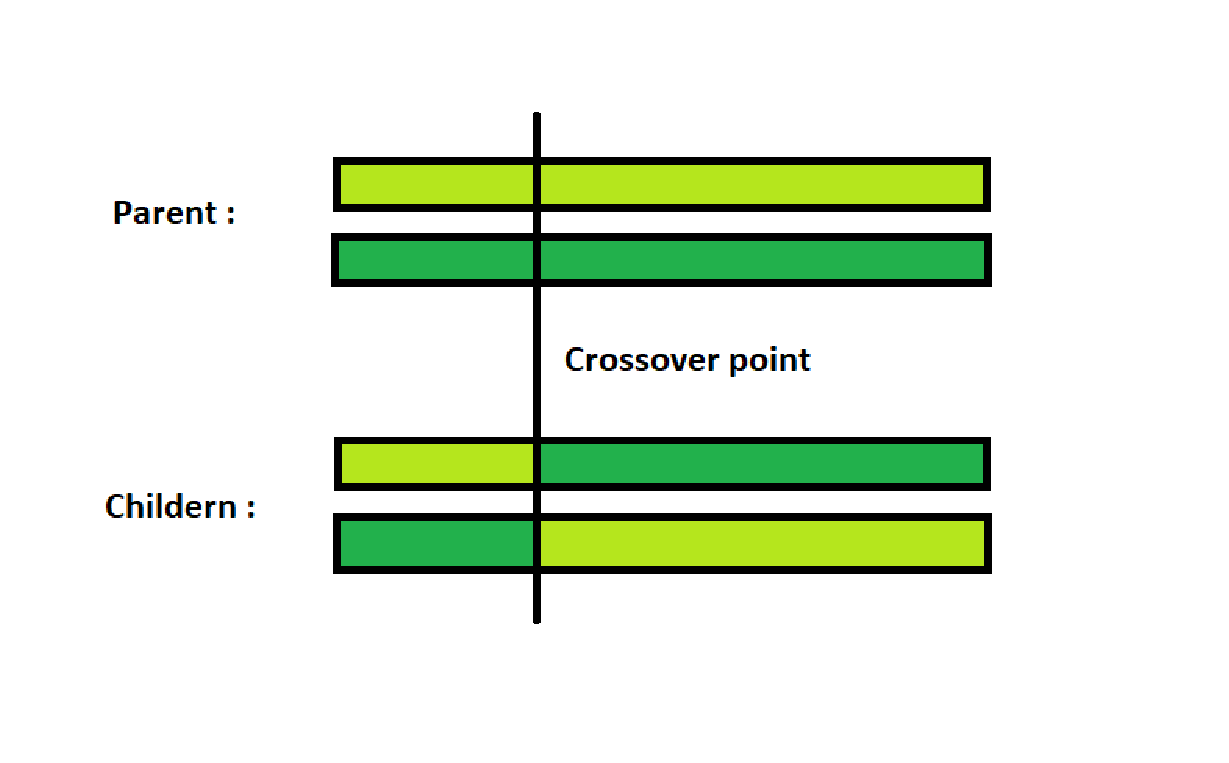
\includegraphics[width=0.8\textwidth]{figures/single_crossover}
	\caption{An example of single point crossover}
\end{figure}

\subsubsection{Uniform crossover}
Each gene (bit) is selected randomly from one of the corresponding genes of the parent chromosomes.
Use tossing of a coin as an example technique.
\begin{figure}[htb] 
	\label{fig:uniform_crossover}
	\centering
	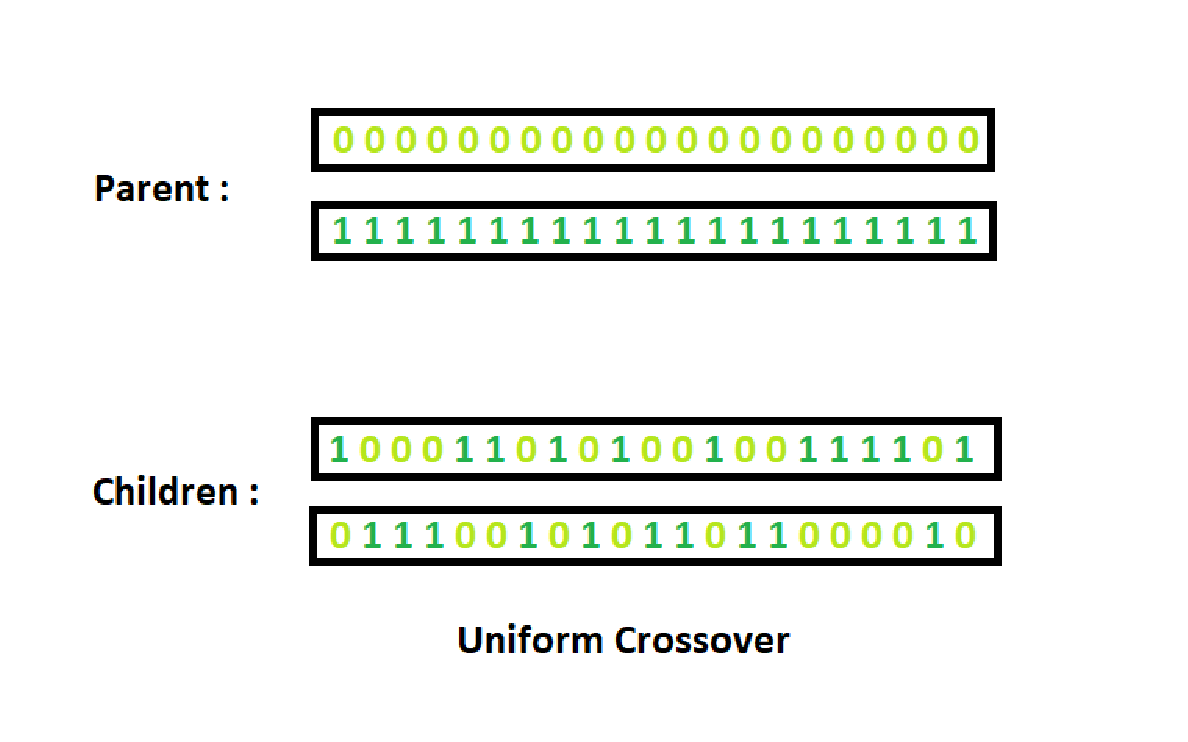
\includegraphics[width=0.8\textwidth]{figures/uniform_crossover}
	\caption{An example of uniform crossover}
\end{figure}


%--------------------------------------------------------------------------------------------------
\subsection{Mutation}
Mutation operator in a genetic algorithm (GA) is usedprimarily as a mechanism for maintaining
diversity in the population.
In contrast to a recombination, a mutation operates on only one evolving population member at a 
time and modifies it independent to the rest of the population members.
Although mutation operator alone may not constitute an efficient search, along with a suitable 
recombination operator, mutation plays an important rolein making the overall search efficient.
For mutation, a bit-wise mutation operator which attempted to mutate every bit (alter the bit to 
its complement) with a probability independently to the outcome of mutationton other bits.
Parametric studies have shown that a mutation probability of $p_{m}= 1/L$ (where $L$ is the total
number of bits used to represent all variables) performed the best.
Researchers have realized that there are certain shortcomings of using a BGA to solve 
real-parameteroptimization problems. One of the reasons was the artificial discreteness associated
with the coding mech-anism and the second was the biasness of mutated solutions towards certain
parts of the search space.
Starting early 1990s, real-parameter GAs (RGAs) were suggested. 
For RGAs, several mutation operators are also suggested.
\subsubsection{Random Mutation}
\subsubsection{Polynomial Mutation}
\subsubsection{Gaussian Mutation}


%--------------------------------------------------------------------------------------------------
\subsection{Elite}

%====================================================================================================
\section{Neuroevolution}

%--------------------------------------------------------------------------------------------------
\subsection{Deep neural networks}
Neuroevolution (NE), the artificial evolution of neural networks using genetic algorithms, 
has shown great promise in complex reinforcement learning tasks. 
Neuroevolution searches through the space of behaviors fora network that performs well
at a given task.
This approach to solving complex controlproblems represents an alternative to statistical
techniques that attempt to estimate theutility of particular actions in particular states
of the world.
Past studies have shown NE to be faster and more efficient than reinforcement learning methods
such as Adaptive Heuristic Critic and Q-Learning on single pole balanc-ing and robot arm control
BecauseNE searches for a behavior instead of a value function, it is effective in problems with
continuous and high-dimensional state spaces.
In addition,  memory is easily repre-sented through recurrent connections in neural networks,
making NE a natural choicefor learning non-Markovian tasks.

%--------------------------------------------------------------------------------------------------
\subsection{Neuroevolution for agumented topologies}

